\documentclass[a4paper]{article}
\usepackage[english]{babel}
\usepackage{amsmath}
\usepackage{graphicx}
\usepackage{placeins}

\title{Building Evacuation}
\author{Maarten de Jonge \\
        Edwin Odijk \\
        Roelof van der Heijden}

\begin{document}

\maketitle

\section{Introduction}
In this report we simulate people escaping from a burning building using the BDI framework. We create an environment with people and fire randomly distributed throughout the building. People randomly walk through the building until they spot fire, at which point they try to run towards the escape and alarm any others they meet along their way. The simulation ends when all people either escaped or died in a fire.
Using this simulation, we aim to find what affects the speed and survival rate of such an evacuation.

\section{Environment}
\FloatBarrier
The simulation environment is a 33x33 grid, representing an office space (Figure
\ref{fig:office}). The walls (black tiles) were hand-drawn to craft a somewhat
realistic layout of rooms and hallways. One exit (green tile) is placed
randomly, as well as a variable number of initial fires (red tiles). Care is
taken to ensure the exit is reachable, i.e. it is not inside a wall or on fire.

\begin{figure}[h!]
  \centering
  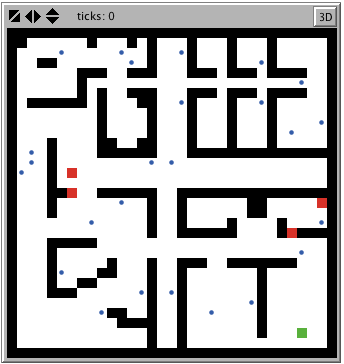
\includegraphics[width=0.5\textwidth]{office.png}
  \label{fig:office}
  \caption{The office layout, with random fires and exit}
\end{figure}

A variable amount of people (ranging from 1 to 25) is spawned, again making sure
not to doom them by spawning them inside walls or fires. At each tick of the
simulation, 

\subsection{Agents}
The agents in this simulation are people trying to escape from the building while avoiding fire. In the BDI framework, they have:
\begin{itemize}
\item Beliefs: Layout of the building, locations of fire, location of exit, locations of other agents
\item Desires: Roam (when no fire is spotted), Find exit, Escape, Alarm others
\item Intentions: Move towards exit, Move away from fire, Move towards other agent, Alarm other agent
\end{itemize}
Agents have the following properties:
\begin{itemize}
\item Whether they are aware of fire.
\item Whether they may/may not pass through eachother.
\item Detection radius for fire.
\item Communication radius to alarm other agents.
\item Whether they prioritize helping other or escaping.
\end{itemize}

When an agent spots fire, he becomes aware of the fire. Whenever they encounter another agent within their communication radius, they will inform them of all fire tiles they know.

\FloatBarrier
\section{Experiments}
\begin{itemize}
\item Can we prevent traffic jam behaviour?
\item How much do the following properties affect overall survival rate?
\begin{itemize}
\item Rate at which fire spreads
\item Whether agents have prior knowledge of exit locations
\item The ratio between agents that prioritize saving themselves over saving others
\end{itemize}
\end{itemize}

\section{Results}

\section{Conclusion}

\end{document}